\documentclass[conference]{IEEEtran}

\usepackage{cite}
\usepackage{amsmath,amssymb,amsfonts}
\usepackage{algorithmic}
\usepackage{graphicx}
\usepackage{textcomp}
\usepackage{xcolor}
\def\BibTeX{{\rm B\kern-.05em{\sc i\kern-.025em b}\kern-.08em
    T\kern-.1667em\lower.7ex\hbox{E}\kern-.125emX}}
\begin{document}

\title{Photogallery, un'applicazione a microservizi}

\author{\IEEEauthorblockN{Matteo Orlando}
\IEEEauthorblockA{\textit{Corso di laurea magistrale in ingegneria informatica} \\
\textit{Università di Tor Vergata, Roma, Italia}\\ \\
matteo.orlando@students.uniroma2.eu}
}

\maketitle

\begin{abstract}
Questo documento descrive la progettazione e l'implementazione di un sistema distribuito di notifiche per gallerie fotografiche, realizzato come applicazione a microservizi in Go. Gli utenti si organizzano in gallerie, il caricamento di una foto in una galleria attiva una notifica per ogni membro di quella galleria, mentre un moderatore può creare, chiudere e inviare avvisi broadcast per le gallerie di sua proprietà. Il sistema è composto da cinque servizi: un API Gateway, un Gallery Service, un Upload Service, un User Service ed un Notification Service che comunicano tramite gRPC e sono orchestrati con Docker Compose su una singola istanza Amazon EC2. Il Gallery Service applica il pattern Command Query Responsibility Segregation (CQRS) per separare le operazioni di scrittura da quelle di lettura, mentre l'Upload Service si protegge da eventuali guasti del Gallery Service tramite l'implementazione del pattern circuit breaker. La distribuzione degli eventi è disaccoppiata tramite RabbitMQ e il Notification Service inoltra gli eventi ai sottoscrittori attivi tramite Server-Sent Events (SSE), utilizzando un livello di broadcast Redis Pub/Sub. In questo modo, il sistema mantiene un comportamento corretto anche quando viene scalato su più repliche. Il documento descrive le motivazioni architetturali, le scelte concrete di implementazione, la suite di test realizzata ed i compromessi operativi osservati durante l'esecuzione dello stack con Docker Compose.
\end{abstract}
\begin{IEEEkeywords}
microservizi, gRPC, CQRS, Circuit Breaker, RabbitMQ, Docker Compose
\end{IEEEkeywords}
\section{Introduction}
Una piattaforma di condivisione di foto o quello che in grande dimensioni prenderebbe il nome di social network, è un contesto naturale per l'impiego di un architettura a microservizi e studiarne i trade-off, in quanto combina tre workload con caratteristiche molto differenti tra loro in un unico ambito: operazioni CRUD sugli utenti delle gallerie ed il contenuto di esse, una grossa richiesta in upload e fan-out a bassa latenza di eventi real-time. Questo progetto implementa tale sistema con l'obiettivo di applicare in maniera completa alcuni dei temi affrontati durante il corso di \textit{Sistemi Distribuiti} quali: remote procedure calls (RPC) e pattern architetturali come CQRS e circuit breaker. I requisiti funzionali sono essenzialmente molto semplici: un utente può registrarsi come un utente tradizionale o un moderatore. Un moderatore può creare, chiudere e cancellare gallerie e può mandare in broadcast messaggi speciali ai membri delle proprie gallerie. Qualunque utente autenticato può unirsi ad una galleria aperta e caricare foto al suo interno e ogni upload avvenuto con successo, produce una notifica che viene consegnata a tutti i membri correnti di tale galleria. I requisiti non funzionali che motivano molte delle scelte architetturali sono:
\begin{enumerate}
\item il sistema deve essere implementato in Go
\item la comunicazione tra i servizi deve utilizzare RPC
\item l'applicazione deve essere capace di scalare e va testato il suo funzionamento
\item il deployment dell'applicazione deve avvenire tramite Docker Compose su un'istanza EC2 di AWS
\end{enumerate}
Il restante contenuto di questo report è organizzato come segue: la sezione II riassume i concetti di background su cui è stato sviluppato il progetto. La sezione III presenta la progettazione ad alto livello del progetto. La sezione IV descrive nel concreto l'implementazione di ogni servizio tra cui, circuit breaker, il pattern CQRS e la pipeline di notifica.La sezione V presenta le metodologie ed i risultati di testing. La sezione VI tratta i trade-off ed i limiti del design scelto. La sezione VII presenta le conclusioni.
\section{BACKGROUND}
\subsection{Microservizi, Database per service e gRPC}
Un'architettura a microservizi decompone un'applicazione in un insieme di servizi indipendenti debolmente accoppiati, che cooperano tra loro. Ogni microservizio che necessita di mantenere dati persistenti ha la proprietà di un database dedicato che è accessibile attraverso la sua API, difatti realizzando così il pattern Database per service. Questo progetto utilizza gRPC come meccanismo di comunicazione tra i servizi. gRPC sfrutta Protocol Buffers come \textit{Interface Definition Language} per generare a partire da file \textit{.proto}, il codice sia del client che del server. Inoltre offre nativamente RPC con streaming dal client al server, dal server al client e bidirezionale ed utilizza il protocollo HTTP/2 per trasporto efficiente. Il progetto si basa su queste funzionalità per le richieste REST ma anche per l'upload delle foto suddiviso in blocchi e per il flusso di notifiche di lunga durata\cite{b3,b5,b18}.
\subsection{CQRS}
Il pattern \textit{Command Query Responsibility Segregation} (CQRS) separa il modello utilizzato per modificare lo stato cioè i comandi, dal modello utilizzato per leggerlo, le query. Anche senza database fisicamente separati o l'implementazione di una replica read-only, suddividere le due responsabilità in interfacce repository distinte mantiene isolati gli invarianti del lato di scrittura dalle esigenze del lato di lettura, permettendo di effettuare operazioni di lettura e scrittura in maniera efficiente e al coltempo rendere possibile evolvere o scalare i due percorsi in modo indipendente in futuro\cite{b1}.
\subsection{Circuit Breaker}
Il pattern \textit{Circuit Breaker} protegge un servizio dai guasti a cascata quando una dipendenza a valle diventa lenta o non disponibile. Un interruttore monitora i fallimenti consecutivi e passa attraverso tre stati: chiuso, dove le chiamate vengono inoltrate, aperto, dove le chiamate vengono rifiutate immediatamente e semiaperto, in cui dopo un periodo di "cooldown" viene consentita una singola chiamata di prova per verificare il ripristino. In questo modo si evita di aggiungere ulteriore carico e latenza a una dipendenza già in difficoltà e si offre ai chiamanti un errore rapido e prevedibile, invece di una richiesta bloccata indefinitamente\cite{b2}.
\subsection{RabbitMQ e Redis}
Il disaccoppiamento tra il servizio che produce un evento come l'upload di una foto, e i servizi che devono reagire a tale evento viene comunemente realizzato tramite un message broker. Questo progetto utilizza RabbitMQ come bus di eventi durevole affiancato dal registro in-memory Redis per inoltrare gli eventi già passati attraverso il broker a numerosi client connessi contemporaneamente, distribuiti su più repliche stateless\cite{b7,b8}.
\subsection{MinIO}
MinIO è un object store compatibile con l'API S3 di Amazon, distribuibile come singolo container. Espone la stessa semantica a oggetti di S3 (bucket, chiavi, policy). Viene utilizzato per l'archiviazione durevole delle foto caricate dagli utenti. In particolare, l'Upload Service vi scrive l'immagine assemblata al termine dello stream gRPC, mentre il Gateway e il frontend consumano direttamente gli URL pubblici restituiti da MinIO per servire le immagini al browser, senza passare per i microservizi\cite{b9}.
\section{DESIGN DELLA SOLUZIONE}
\subsection{Decomposizione servizi}
I requisiti informali individuati a monte della realizzazione del progetto erano: (i) esistono diverse gallerie a cui gli utenti possono partecipare per caricare immagini; (ii) il caricamento di una foto attiva una notifica per ogni membro della galleria di appartenenza; e (iii) esiste un ruolo di moderatore, con la facoltà di creare e chiudere gallerie e di inviare avvisi broadcast speciali. Questi requisiti si riconducono naturalmente a quattro capacità: gestione dell'identità e delle autorizzazioni, ciclo di vita e gestione dei membri delle gallerie, acquisizione e archiviazione delle foto e distribuzione delle notifiche. Tali capacità sono diventate i quattro servizi principali descritti di seguito, oltre a un quinto servizio, l'API Gateway, che li espone in modo uniforme tramite protocollo HTTP.
\begin{itemize}
\item \textbf{API Gateway}: traduce le chiamate HTTP/REST del client browser in chiamate gRPC. Integra grpc-gateway per i servizi User e Gallery in modo che le annotazioni nei rispettivi file .proto generino direttamente gli URL REST e un livello basato su Gin per il caricamento di foto ed il flusso di notifiche basato su Server-Sent Events.
\item \textbf{User Service}: gestisce l'identità degli utenti ovvero: registrazione, accesso e emissione/validazione dei JWT. Le password vengono sottoposte a hashing con bcrypt; tutti gli altri servizi si fidano al token JWT anziché verificare nuovamente le credenziali.
\item \textbf{Gallery Service}: gestisce il ciclo di vita delle gallerie tramite creazione, chiusura ed eliminazione e l'appartenenza a esse. Internamente è suddiviso in un lato comandi e un lato query, secondo il pattern CQRS.
\item \textbf{Upload Service}: accetta una foto trasmessa tramite streaming dal client, la salva in MinIO (un object store compatibile con S3), verifica l’appartenenza dell’utente alla galleria tramite una chiamata al Gallery Service protetta da un circuit breaker, registra il caricamento in PostgreSQL e pubblica un evento di caricamento su RabbitMQ.
\item \textbf{Notification Service}: consuma gli eventi da RabbitMQ, determina quali utenti devono essere notificati per ciascun evento e invia le notifiche a ogni membro iscritto attivo tramite un flusso gRPC server-side di lunga durata, che il Gateway riespone al browser come SSE.
\end{itemize}
\subsection{Comunicazione e proprietà dei dati}
Tutte le chiamate tra servizi utilizzano gRPC, l'unica interfaccia HTTP è il confine tra il Gateway e il browser. Ogni servizio che necessita di un'archiviazione persistente possiede un database PostgreSQL privato, quindi nessun servizio accede direttamente alle tabelle di un altro servizio. Per le query tra servizi ad esempio, la verifica di appartenenza di un utente ad una specifica galleria, vengono sempre eseguite tramite una chiamata gRPC, mai attraverso uno schema condiviso. In questo modo i servizi possono essere distribuiti in modo indipendente e ogni database può essere migrato, scalato o sostituito senza dover coordinare le operazioni con gli altri.
\subsection{Frontend}
Il frontend è realizzato come una Single Page Application in React e adotta il pattern architetturale Flux per separare la gestione dello stato dalla logica di presentazione. L'interfaccia è organizzata in componenti React specializzati nelle diverse funzionalità dell'applicazione, mentre lo stato relativo alle operazioni asincrone e alle risorse visualizzate viene mantenuto nei rispettivi store. Per la gestione delle notifiche in tempo reale viene utilizzato il protocollo Server-Sent Events (SSE). Il browser mantiene una connessione persistente con l'endpoint di notificazione del Gateway e riceve gli eventi prodotti dal Notification Service senza dover effettuare un polling periodico. Quando la connessione viene interrotta, il frontend tenta automaticamente di ristabilirla utilizzando un meccanismo di riconnessione con \textit{exponential backoff}. In questo modo una temporanea indisponibilità del Gateway o del servizio di notificazione non richiede un intervento manuale dell'utente e, contemporaneamente, evita di generare un elevato numero di tentativi ravvicinati durante un guasto prolungato\cite{b14,b19}.
\subsection{Topologia di deployment}
L'intero stack: tre istanze PostgreSQL, RabbitMQ, Redis, MinIO, i cinque microservizi e un frontend React a pagina singola, posto dietro nginx vengono definiti all'interno di un unico file \textit{docker-compose.yaml} e distribuito su un’unica istanza EC2. Ogni servizio Go dispone di un proprio Dockerfile multi-stage che compila un binario statico e lo copia in un'immagine Alpine minimale, mantenendo ridotte le dimensioni delle immagini e la superficie di attacco. I controlli all'avvio dei servizi fanno in modo che, per esempio, il Gallery Service non accetti traffico finché la sua dipendenza PostgreSQL non segnala di essere operativa\cite{b6}.
\begin{figure}[t]
\centering
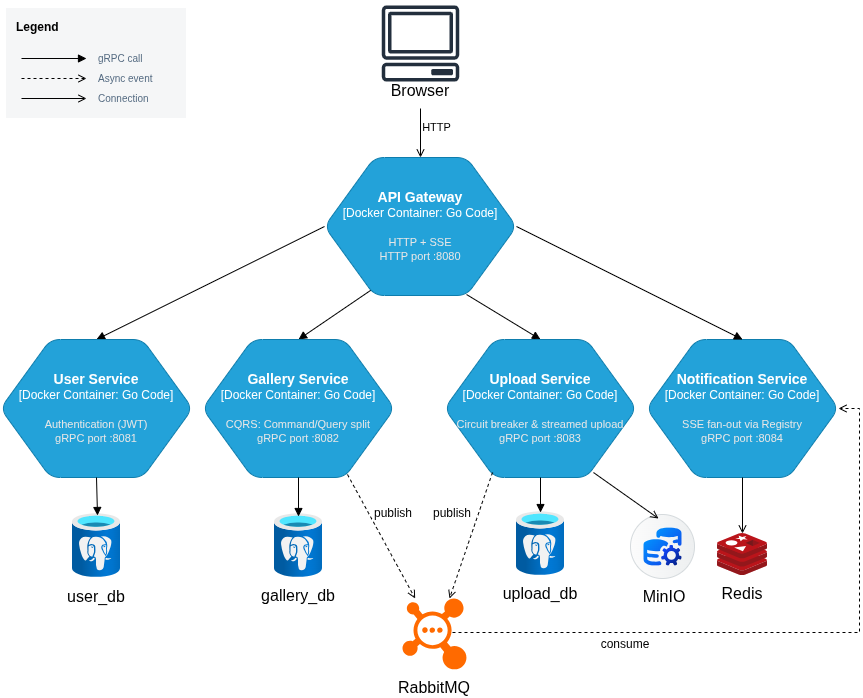
\includegraphics[width=\columnwidth]{architettura.png}
\caption{Architettura complessiva del sistema e principali flussi di comunicazione tra i componenti.}
\label{fig:architettura}
\end{figure} 	
\section{DETTAGLI IMPLEMENTATIVI}
\subsection{Buf}
La definizione delle interfacce tra i microservizi è basata su Protocol Buffers e il progetto utilizza \textit{Buf} per gestire in modo centralizzato la validazione e la generazione del codice a partire dai file \textit{.proto}. I file \textit{buf.yaml}, \textit{buf.gen.yaml} e \textit{buf.lock} descrivono rispettivamente il modulo protobuf del progetto, i plugin e le opzioni utilizzate durante la generazione e le versioni delle dipendenze protobuf risolte. In questo modo la generazione non dipende da una sequenza di comandi \textit{protoc} specifici per ogni servizio, ma può essere riprodotta tramite un unico workflow basato su \texttt{buf generate}. La configurazione genera gli artefatti necessari al progetto Go, inclusi i messaggi Protocol Buffers, gli stub gRPC e il codice del grpc-gateway. Buf costituisce quindi un punto unico per mantenere coerenti codice generato e dipendenze tra i diversi servizi\cite{b12}.
\subsection{GORM}
Per l'accesso ai database PostgreSQL i servizi che necessitano di persistenza utilizzano GORM, un ORM per Go che permette di rappresentare le tabelle tramite strutture Go e di eseguire le operazioni sul database attraverso un'API tipizzata. Nel progetto GORM viene utilizzato principalmente all'interno del livello repository, mantenendo così i dettagli di persistenza separati dalla logica applicativa. Questa separazione consente ai service di dipendere da interfacce repository invece che direttamente dal database e rende possibile sostituire o modificare l'implementazione della persistenza senza modificare la logica dei service.\cite{b15}.
\subsection{GoMock}
La separazione tramite interfacce è sfruttata anche nei test grazie a GoMock. Le dipendenze esterne dei componenti sottoposti a test, come repository, client gRPC, publisher RabbitMQ e sistemi di storage, vengono rappresentate tramite interfacce e sostituite nei test da mock generati automaticamente. Il mock definisce le chiamate attese e permette al test di verificare non solo il valore restituito dalla dipendenza, ma anche che una determinata operazione venga invocata con gli argomenti corretti e nel numero di volte previsto. I test possono quindi concentrarsi sulla logica di business, mentre le integrazioni con i componenti esterni vengono verificate nelle suite di test di integrazione.\cite{b16}.
\subsection{Gin e grpc-gateway}
Il Gateway adotta due meccanismi complementari. Per le API User e Gallery viene utilizzato grpc-gateway, che genera un reverse proxy HTTP/JSON a partire dai contratti gRPC definiti nei file Protocol Buffers. Le annotazioni \texttt{google.api.http} associano le RPC ai metodi e alle route HTTP corrispondenti. Anche la conversione degli errori è demandata al runtime del grpc-gateway, che permette di tradurre gli status gRPC nei corrispondenti codici HTTP\cite{b3,b11}. Per le funzionalità che non si adattano al modello unary di gRPC viene invece utilizzato Gin. In particolare, il router Gin gestisce l'upload delle immagini e l'endpoint SSE per le notifiche. Il Gateway mantiene così un ruolo di adattatore: grpc-gateway viene utilizzato dove la corrispondenza tra RPC e HTTP è diretta, mentre Gin fornisce il controllo necessario per le route HTTP con semantica più specifica\cite{b4,b11}.
\subsection{Autenticazione}
L'autenticazione è gestita centralmente dal \textit{User Service}, che si occupa della registrazione degli utenti, del login e dell'emissione dei token JWT. Durante la registrazione, la password non viene memorizzata in chiaro, ma viene trasformata tramite hashing con bcrypt. In seguito al login o registrazione, il servizio genera un JWT contenente le informazioni necessarie per identificare il chiamante e determinarne il ruolo. Il token viene quindi utilizzato dal client nelle successive richieste senza dover trasmettere nuovamente le credenziali. L'autenticazione viene verificata principalmente all'ingresso dei servizi gRPC tramite un \textit{interceptor}. L'interceptor estrae il JWT dalle credenziali della richiesta, ne verifica la validità e rende disponibili al metodo RPC le informazioni relative al chiamante. Questo approccio evita di duplicare il controllo del token all'interno di ogni singolo handler e permette di mantenere separata la responsabilità di autenticazione dalla logica applicativa.
\subsection{CQRS in Gallery Service}
Il Gallery Service espone due interfacce Go interne, CommandRepository e QueryRepository, ciascuna supportata da una propria implementazione basata su GORM\cite e operante sulla stessa istanza di Postgres, gallery\_db. CommandRepository gestisce CreateGallery, UpdateGallery, DeleteGallery, JoinGallery e LeaveGallery; QueryRepository gestisce GetGallery, ListGalleries, ListGalleriesByMember, ListMembers e IsMember. Un CommandService e un QueryService incapsulano questi repository applicando la logica di business: per esempio, DeleteGallery e CloseGallery verificano entrambi che il chiamante sia il moderatore della galleria prima di modificare qualsiasi dato, mentre JoinGallery rifiuta le richieste di partecipazione a una galleria chiusa. Il gestore gRPC (api/grpc.go) dipende soltanto da due interfacce ridotte, CommandRunner e QueryRunner, realizzate per effettuare unit test su entrambi i lati singolarmente tramite mock generati GoMock\cite{}, senza utilizzare un database reale. Ogni gestore di comandi che produce un effetto collaterale degno di essere trasmesso come: GalleryClosed o ModeratorAlert, pubblica un evento su RabbitMQ all’interno di una goroutine in background, dopo il completamento della transazione di scrittura sul database. In questo modo, un broker lento o degradato non aggiunge latenza alla richiesta sincrona.
\subsection{Circuit Breaker nell'Upload Service}
Ogni chiamata UploadPhoto deve verificare, tramite la RPC IsMember del Gallery Service, che il chiamante appartenga alla galleria di destinazione e che la galleria sia ancora aperta. Poiché si tratta di una dipendenza sincrona da un altro servizio, attiva per ogni richiesta, essa è racchiusa in un circuit breaker a tre stati implementato manualmente (internal/upload/circuitbreaker.go). Il breaker si apre dopo un numero configurabile di errori consecutivi (tre nella configurazione di default) rimane aperto per un timeout di ripristino fisso (dieci secondi) e quindi consente il passaggio di una sola chiamata di prova nello stato semiaperto. Questo comportamento è protetto da un flag booleano e da un mutex, così che, anche sotto carico concorrente, una sola goroutine alla volta possa verificare il ripristino mentre tutti gli altri chiamanti concorrenti vengono rifiutati immediatamente con uno stato gRPC UNAVAILABLE, invece di aggiungersi al carico di una dipendenza che è ancora in fase di verifica.
\subsection{Upload delle foto e streaming notifiche}
\textit{UploadPhoto} è una RPC con streaming dal client: il primo messaggio dello stream contiene \textit{UploadMetadata} (ID della galleria, nome del file, tipo di contenuto e dimensione dichiarata), mentre ogni messaggio successivo contiene un blocco grezzo di byte dell'immagine di dimensione fissa. In questo modo si evita di caricare un'immagine completa all'interno di un singolo messaggio gRPC, il che sarebbe computazionalmente inefficiente. Il server impone un limite massimo di 25 MB, sulla dimensione massima della foto, impedendo così che un client malevolo o difettoso provochi una crescita illimitata della memoria. Quando lo stream viene concluso, il server verifica l'appartenenza tramite il circuit breaker descritto sopra, salva l'immagine assemblata in MinIO, memorizza una riga Record interrogabile in PostgreSQL, una riga per ogni foto, indicizzata per galleria e per ID della foto e pubblica un evento \textit{PhotoUploaded} senza attendere la risposta. L'istanza di Postgres è necessaria dal momento in cui senza di essa, non sarebbe possibile utilizzare repliche di Upload Service e non ci sarebbe persistenza tra un restart e l'altro dell'applicazione.
\subsection{Distribuzione delle notifiche e scalabilità orizzontale}
Il Registry del Notification Service mantiene un indice in memoria, specifico per ogni replica, dei sottoscritti SSE connessi. L'indice è organizzato prima per galleria e separatamente per utente, così che un singolo utente con diverse schede del browser aperte venga tracciato come un insieme di connessioni indipendenti, aggiungibili o rimovibili singolarmente dall'insieme degli iscritti di una galleria. Poiché RabbitMQ consegna ogni evento a un solo consumer e il Notification Service è progettato per essere eseguito con più repliche, un'implementazione superficiale notificherebbe soltanto i membri connessi alla replica che, casualmente, ha ricevuto e consumato una determinata consegna da RabbitMQ. L'implementazione attuale evita questo problema tramite il data store Redis, che implementa il paradigma Pub/Sub. La replica il cui Consumer consuma un evento da RabbitMQ ripubblica la notifica risultante, su un canale Redis condiviso, al quale sono iscritte tutte le repliche. Ogni replica applica quindi l'evento al proprio Registry locale, compresa la replica che lo ha pubblicato originariamente. In questo modo la consegna è corretta indipendentemente dalla replica che gestisce la connessione attiva di un determinato utente.
\subsection{API Gateway}
Il Gateway non contiene logica di business: per User e Gallery registra semplicemente i gestori HTTP generati da grpc-gateway sulle corrispondenti connessioni client gRPC, in modo che ogni route REST venga derivata meccanicamente dalle annotazioni `google.api.http` presenti nei file \textit{.proto}. Il caricamento e il flusso delle notifiche sono invece gestiti da un router Gin di dimensioni ridotte, poiché il caricamento di file multiparti e gli eventi Server-Sent Events non rientrano nel modello unary basato su JSON di grpc-gateway. I codici di stato gRPC restituiti da qualsiasi servizio backend vengono convertiti nel corrispondente stato HTTP tramite runtime.HTTPStatusFromCode. Per esempio, quando il circuit breaker scatta, il browser riceve '503 Service Unavailable' invece di un generico errore 500.
\section{RISULTATI}
\subsection{Continuous Integration e test unitari}
Il progetto include una pipeline di \textit{Continuous Integration} realizzata tramite GitHub Actions, eseguita automaticamente in occasione di push e pull request. Lo scopo della pipeline è verificare che ogni modifica possa essere compilata e che la suite di test continui a passare prima che il cambiamento venga considerato integrabile nel ramo principale. La correttezza dei singoli servizi viene verificata tramite test d'unità che simulano ogni dipendenza esterna, repository di database, client gRPC, sistema di archiviazione e publisher dei messaggi, usando GoMock, così che ogni test eserciti esclusivamente la logica di business sottoposta a verifica. Tra gli aspetti verificati rientrano: le regole di autorizzazione e tutte le transizioni del circuit breaker. Il workflow utilizza l'ambiente Go dichiarato dal progetto, recupera le dipendenze e quindi esegue la compilazione del codice e i test dell'intero modulo con \texttt{go test ./...} e raccoglie anche la copertura l'opzione \texttt{-cover}, fornendo un'indicazione quantitativa della parte di codice esercitata dai test.\cite{b17}.
\subsection{Test di integrazione}
Una suite separata di test di integrazione, esercita il sistema come un vero client black-box dell'interfaccia HTTP distribuita. I test registrano utenti reali, creano e utilizzano gallerie reali, caricano immagini di piccole dimensioni generate sinteticamente e verificano le risposte HTTP risultanti e, per il percorso delle notifiche, gli eventi SSE reali vengono osservati durante la trasmissione. Questi test coprono l'intero flusso di partecipazione e notifica, l'autorizzazione riservata al moderatore per le operazioni di eliminazione, chiusura e invio di avvisi, la corretta conversione in codici di stato HTTP di un caricamento rifiutato. Quando vengono eseguiti su un deployment con Docker Compose scalato con più di una replica di un servizio, vengono testati due comportamenti cruciali: (i) un upload reso persistente da una replica è visibile a una query gestita da una replica diversa e (ii) ogni membro riceve un avviso del moderatore, indipendentemente dalla replica di notification-service che gestisce la sua connessione.
\subsection{Load test}
Due generatori di carico Go progettati appositamente (cmd/testupload, cmd/testgallery) applicano carichi di lavoro concorrenti e pesati a un Gateway distribuito e riportano i percentili di latenza per operazione e i tassi di errore, oltre al throughput ed ai valori massimi e minimi del tempo di risposta. Il load test per l'upload (cmd/testupload) può arrestare e riavviare il servizio gallery-service a un offset configurato dall'inizio dell'esecuzione. Questa funzionalità è pensata per essere confrontata con le righe di log del circuit breaker dell'Upload Service, così da verificare che il breaker si apra poco dopo la scomparsa della dipendenza e si richiuda dopo il suo ripristino. I risultati dei due generatori di carico sono riportati nelle Figure~\ref{fig:load-gallery} e~\ref{fig:load-upload}, rispettivamente per il Gallery Service e per l'Upload Service. Il confronto considera esecuzioni con una sola replica e con tre repliche dei servizi. In generale, l'esecuzione con più repliche mostra un throughput più elevato e una percentuale di errori inferiore rispetto alla configurazione con una sola replica. Questi risultati devono tuttavia essere interpretati nel contesto dell'ambiente di prova: le prestazioni dipendono dalle dimensioni dell'istanza EC2, dal numero effettivo di repliche attive per ciascun servizio e dal carico generato durante la misurazione.
\begin{figure}[t]
\centering
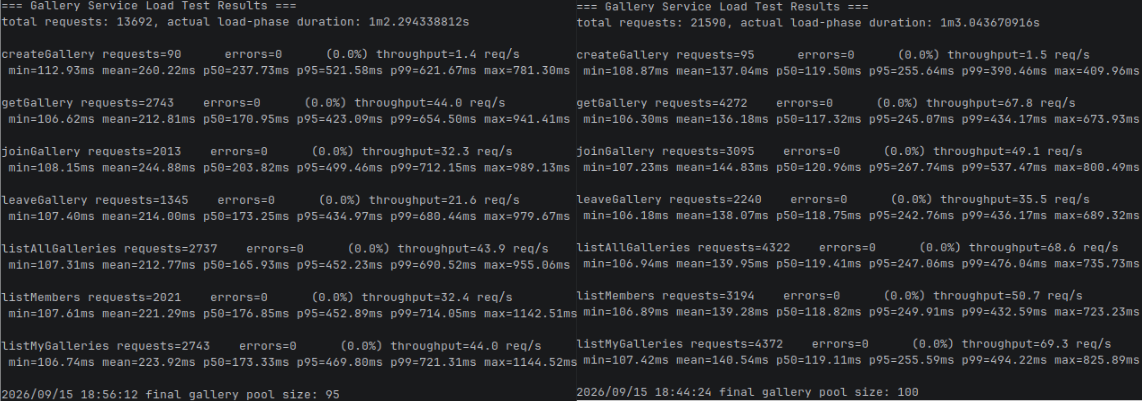
\includegraphics[width=\columnwidth]{load_test_gallery.png}
\caption{Risultati del load test per il Gallery Service.}
\label{fig:load-gallery}
\end{figure}
\begin{figure}[t]
\centering
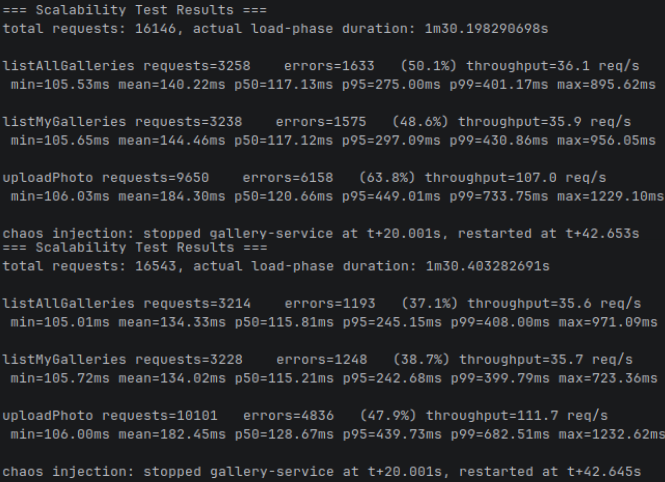
\includegraphics[width=\columnwidth]{load_test_upload.png}
\caption{Risultati del load test per l'Upload Service.}
\label{fig:load-upload}
\end{figure}
\section{DISCUSSIONE}
\subsection{Implementazioni efficaci}
L'architettura a microservizi ha permesso di separare chiaramente le responsabilità dei diversi componenti del sistema, rendendo l'applicazione modulare e facilitando lo sviluppo e il testing dei singoli servizi. L'adozione del pattern CQRS nel Gallery Service ha consentito di mantenere separati i percorsi relativi alle operazioni di scrittura e di lettura, rendendo in particolare più semplice isolare e testare la logica di business. Il circuit breaker implementato nell'Upload Service ha invece introdotto un meccanismo di resilienza nei confronti delle dipendenze esterne, limitando l'effetto di eventuali malfunzionamenti del Gallery Service. Un ulteriore elemento importante è rappresentato dalla combinazione di RabbitMQ e Redis per la gestione delle notifiche. RabbitMQ permette di distribuire gli eventi prodotti dai servizi, mentre Redis consente di propagare tali eventi tra le diverse repliche del Notification Service. In questo modo, il sistema può continuare a gestire correttamente le notifiche anche quando il servizio viene scalato orizzontalmente. L'adozione della CI ha inoltre permesso di automatizzare build e test, aspetto importante in un'architettura composta da più servizi, dove una modifica locale può avere effetti sugli altri componenti.
\subsection{Limitazioni e compromessi}
Nonostante i meccanismi di resilienza introdotti, l'implementazione presenta alcune limitazioni. La principale riguarda la pubblicazione degli eventi: essi vengono pubblicati in una goroutine in background dopo il completamento della transazione, evitando di aggiungere latenza alla richiesta sincrona. Tuttavia, un eventuale arresto del servizio tra il commit del database e la pubblicazione dell'evento può causare la perdita della notifica. L'uso di RabbitMQ accoppiato a Redis Pub/Sub introduce una piccola quantità di lavoro ridondante, poiché ogni replica deve applicare localmente il filtraggio degli eventi ricevuti. Anche il Registry del Notification Service rappresenta un compromesso progettuale. Lo stato delle connessioni viene mantenuto in memoria e deve essere ricostruito quando un client si riconnette. Questa soluzione mantiene l'implementazione semplice, ma il costo della ricostruzione può aumentare all'aumentare del numero di gallerie e membri coinvolti. Un'ulteriore limitazione riguarda l'infrastruttura utilizzata per la distribuzione. RabbitMQ, Redis e le tre istanze PostgreSQL non sono attualmente replicate e rappresentano quindi potenziali single point of failure. Inoltre, l'utilizzo di Docker Compose su una singola istanza EC2 semplifica la configurazione e la riproducibilità dell'ambiente, ma non permette di ottenere una distribuzione realmente su più host e quindi un livello di disponibilità paragonabile a quello di un ambiente di produzione. Infine, i test di carico hanno mostrato un miglioramento del throughput e una riduzione della percentuale di errori utilizzando più repliche, ma come anticipato, i risultati dipendono dalle dimensioni dell'istanza EC2, dal numero di repliche e dal numero di esecuzioni effettuate. Per una valutazione sperimentale più robusta sarebbe necessario ripetere ciascuna configurazione più volte e riportare intervalli di confidenza.
\subsection{Possibili estensioni}
Una prima estensione consiste nell'introduzione di meccanismi più avanzati, per eliminare problemi di consistenza legati alla pubblicazione degli eventi, andando a rendere atomiche la modifica dello stato e la registrazione dell'evento da pubblicare. Un secondo possibile sviluppo riguarda l'evoluzione del modello CQRS verso una separazione più completa del modello di lettura, attraverso una replica dedicata alle query. Questo permetterebbe di sfruttare maggiormente i vantaggi della separazione tra command e query già introdotta nel Gallery Service. Dal punto di vista infrastrutturale, una possibile evoluzione consiste nel passaggio da Docker Compose a Kubernetes. Tale soluzione permetterebbe di gestire più facilmente il deployment su più host, la replica dei servizi, i rolling update e i meccanismi di liveness e readiness. In un ambiente di questo tipo sarebbe inoltre possibile integrare infrastrutture gestite o replicate per PostgreSQL, RabbitMQ e Redis. Infine, il sistema potrebbe essere esteso con strumenti di monitoraggio e logging distribuito, in modo da facilitare l'analisi del comportamento dei microservizi e l'individuazione dei problemi in un ambiente realmente distribuito.
\section{Conclusioni}
Il progetto ha portato alla realizzazione di un sistema distribuito per la gestione di una galleria fotografica, composto da cinque microservizi sviluppati in Go e comunicanti tramite gRPC. L'architettura combina comunicazione sincrona e asincrona attraverso gRPC e RabbitMQ, mentre PostgreSQL, Redis e MinIO vengono utilizzati per la gestione rispettivamente dei dati, della propagazione delle notifiche tra repliche e delle immagini. Il sistema permette agli utenti di registrarsi e autenticarsi, partecipare a più gallerie, caricare fotografie e ricevere notifiche in tempo reale. Il ruolo di moderatore consente inoltre di creare e chiudere le gallerie e di inviare messaggi agli utenti interessati. L'adozione di CQRS ha permesso di separare la logica relativa alle operazioni di scrittura da quella delle query, mentre il circuit breaker ha migliorato la resilienza del sistema in presenza di malfunzionamenti delle dipendenze. La combinazione di RabbitMQ, Redis e Server-Sent Events permette inoltre di distribuire le notifiche tra più repliche del Notification Service, consentendo il funzionamento del sistema anche scalando orizzontalmente. L'architettura sviluppata presenta comunque possibilità di evoluzione attraverso l'introduzione di un modello di lettura più evoluto, l'utilizzo di Kubernetes, l'introduzione di infrastrutture replicate e gestite, una maggiore gestione della consistenza e l'integrazione di sistemi di monitoring e distributed logging. Nel complesso, il progetto rappresenta un'applicazione concreta dei principali concetti affrontati nell'ambito dei sistemi distribuiti, funzionale e testabile. I test unitari, i test di integrazione e i test di carico hanno infatti permesso di verificare sia la correttezza delle principali funzionalità sia il comportamento del sistema in condizioni di scalabilità e di guasto simulato, mentre i risultati ottenuti mostrano come l'architettura proposta sia in grado di soddisfare i requisiti funzionali del progetto, fornendo allo stesso tempo una base sulla quale sviluppare ulteriori funzionalità e miglioramenti infrastrutturali.
\begin{thebibliography}{00}
\bibitem{b1}
M. Fowler, ``CQRS,'' \textit{Martin Fowler's Bliki}, Jul. 2011.
[Online]. Available: https://martinfowler.com/bliki/CQRS.html
\bibitem{b2}
M. Fowler, ``Circuit Breaker,'' \textit{Martin Fowler's Bliki}, Mar. 2014.
[Online]. Available: https://martinfowler.com/bliki/CircuitBreaker.html
\bibitem{b3}
gRPC Authors, ``gRPC Documentation,'' 2026.
[Online]. Available: https://grpc.io/docs/
\bibitem{b4}
Gin Authors, ``Gin Web Framework Documentation,'' 2026.
[Online]. Available: https://gin-gonic.com/en/docs/
\bibitem{b5}
Google, ``Protocol Buffers Documentation,'' 2026.
[Online]. Available: https://protobuf.dev/
\bibitem{b6}
Docker Inc., ``Docker Compose Documentation,'' 2026.
[Online]. Available: https://docs.docker.com/compose/
\bibitem{b7}
RabbitMQ Authors, ``RabbitMQ Documentation,'' 2026.
[Online]. Available: https://www.rabbitmq.com/docs
\bibitem{b8}
Redis Ltd., ``Redis Pub/Sub Documentation,'' 2026.
[Online]. Available: https://redis.io/docs/latest/develop/pubsub/
\bibitem{b9}
MinIO, Inc., ``MinIO Documentation,'' 2026.
[Online]. Available: https://min.io/docs/
\bibitem{b11}
gRPC-Gateway Authors, ``gRPC-Gateway Documentation,'' 2026.
[Online]. Available: https://grpc-ecosystem.github.io/grpc-gateway/
\bibitem{b12}
Buf Authors, ``Buf Documentation: How Buf Compares to Protoc,'' 2026.
[Online]. Available: https://buf.build/docs/
\bibitem{b14}
K. Hoffman and D. Nemeth, \textit{Cloud Native Go: Building Web Applications and Microservices for the Cloud with Go and React}.
Boston, MA, USA: Addison-Wesley Professional, 2016. pp. 195-207
\bibitem{b15}
GORM Authors, ``GORM Documentation,'' 2026.
[Online]. Available: https://gorm.io/docs/
\bibitem{b16}
Uber Go Authors, ``GoMock,'' 2026.
[Online]. Available: https://github.com/uber-go/mock
\bibitem{b17}
GitHub, ``Building and testing Go,'' \textit{GitHub Actions Documentation}, 2026.
[Online]. Available: https://docs.github.com/en/actions/tutorials/build-and-test-code/go
\bibitem{b18}
M. Richardson, ``Database per service,'' \textit{Microservices.io}.
\bibitem{b19}
React Authos, ``React,'' 2026. 
[Online]. Available: https://react.dev/learn
\end{thebibliography}

\end{document}
